\documentclass [10pt]{book}
\oddsidemargin=0.0cm
\textwidth=16.5cm
\textheight=22.8cm
\topmargin=-1.0cm
\usepackage[utf8]{inputenc}
\usepackage{booktabs}
\usepackage{fancyhdr}
\usepackage{multicol}
\usepackage{mathtools}% Loads amsmath
\usepackage{flowchart}
\usepackage{xcolor}
\usepackage{lipsum}
\usepackage{graphicx}
\usepackage{float}
\usepackage{geometry}
\renewcommand*\contentsname{Contents}
\definecolor{namecolor}{cmyk}{1,.50,0,.10}
\definecolor{titlepagecolor}{cmyk}{1,.209,0,.831}
\renewcommand{\thesection}{\arabic{section}}
\renewcommand{\headrulewidth}{3pt}% 2pt header rule
\renewcommand{\headrule}{\hbox to\headwidth{%
  \color{titlepagecolor}\leaders\hrule height \headrulewidth\hfill}}
\pagestyle{fancy}
\fancyhf{}
\fancyhead[LE]{\hspace*{-0.2\headwidth}\colorbox{titlepagecolor!20}{\makebox[\dimexpr0.2\headwidth-2\fboxsep][c]{\strut\thepage}}%
               \colorbox{titlepagecolor}{\makebox[\dimexpr\headwidth-2\fboxsep][l]{Section \strut\thesection}}}
\fancyhead[LO]{\colorbox{titlepagecolor}{\makebox[\dimexpr\headwidth-2\fboxsep][r]{Section \strut\thesection}}%
                \colorbox{titlepagecolor!20}{\makebox[\dimexpr0.2\headwidth-2\fboxsep][c]{\strut\thepage}}}
\renewcommand{\headrulewidth}{0pt}
%\lhead{\fancyplain{}{\leftmark }}
%\rhead{\fancyplain{}{Alarm Clock}}
%\renewcommand{\headrulewidth}{1pt}
\lfoot{}
\usepackage{listings}
\usepackage{multicol}

% the following is needed for syntax highlighting
\usepackage{color}
\definecolor{dkgreen}{rgb}{0,0.6,0}
\definecolor{gray}{rgb}{0.5,0.5,0.5}
\definecolor{mauve}{rgb}{0.58,0,0.82}
\lstset{ %
language=[C]{Assembler},      % the language of the code
basicstyle=\scriptsize,         % the size of the fonts that are used for the code
numbers=left,                   % where to put the line-numbers
numberstyle=\tiny\color{gray},  % the style that is used for the line-numbers
stepnumber=1,                   % the step between two line-numbers. If it's 1, each line
% will be numbered
numbersep=5pt,                  % how far the line-numbers are from the code
backgroundcolor=\color{white},  % choose the background color. You must add \usepackage{color}
showspaces=false,               % show spaces adding particular underscores
showstringspaces=false,         % underline spaces within strings
showtabs=false,                 % show tabs within strings adding particular underscores
frame=single,                   % adds a frame around the code
rulecolor=\color{white},        % if not set, the frame-color may be changed on line-breaks within not-black text (e.g. commens (green here))
tabsize=2,                      % sets default tabsize to 2 spaces
captionpos=b,                   % sets the caption-position to bottom
breaklines=true,                % sets automatic line breaking
breakatwhitespace=false,        % sets if automatic breaks should only happen at whitespace
title=\lstname,                 % show the filename of files included with \lstinputlisting;
% also try caption instead of title
keywordstyle=\color{blue},          % keyword style
commentstyle=\color{gray},       % comment style
stringstyle=\color{mauve},         % string literal style
escapeinside={\%*}{*)},            % if you want to add a comment within your code
morekeywords={*,...}               % if you want to add more keywords to the set
}
% facilitates the creation of memory maps. Start address at the bottom, end address at the top.
% Addresses will be print with a leading '0x' and in upper case.
% syntax: \memsection{end address}{start address}{height in lines}{text in box}
\newcommand{\memsection}[4]{
  \bytefieldsetup{bitheight=#3\baselineskip}	% define the height of the memsection
  \bitbox[]{8}{
    \texttt{0x\uppercase{#1}}	 % print end address
    \\ \vspace{#3\baselineskip} \vspace{-2\baselineskip} \vspace{-#3pt} % do some spacing
    \texttt{0x\uppercase{#2}} % print start address
  }
  \bitbox{16}{#4} % print box with caption
}

% Start the document
\begin{document}
\begin{titlepage}
\newgeometry{left=7.5cm} %defines the geometry for the titlepage
\pagecolor{titlepagecolor}
\noindent
\color{white}
\makebox[0pt][l]{\rule{1.3\textwidth}{1pt}}
\par
\noindent
\textbf{\textsf{University at Buffalo}} \textcolor{titlepagecolor!20}{\textsf{}}
\vfill
\noindent
{\huge \textsf{Stratus Print Node }}
\vskip\baselineskip
\noindent
\textsf{User Documentation - Spring 2016}
\end{titlepage}

  \pagecolor{white}

  \tableofcontents
  %Body

  \newpage
  \section{Set up}
    \begin{enumerate}
      \item Ensure the node is plugged in and the switch is in the "ON" position.
      The red light will be illuminated on the node when there is power. If the node
      has already been activated on the hub you are done or else move to step 2.

      \item If this is the first time the node is being connected to the hub.
      You will need to activate it on the hub. To do this you will need a device
      capable of connecting to a wi-fi network, such as a smart phone. Under networks
      you should see a network called "SetUpGadget\_FPFDHI". Note that the "FPFDHI"
      can be any sequence of letters and is specific to the node. Connect to that network.
      Once connected you may get a warning that the network does not have access
      to the internet. That is normal proceed anyway.

      \item Open your browser and navigate to "192.168.4.1". This will bring up
      a wifi log in page. Here you will type in the hub information.
      \begin{center}
      
\includegraphics[scale=1]{images/ip-enter.png}
    \end{center}

      \item For the wifi name type "StratusPrint" and for the password "FusRoDah".
      These are the default wifi mane and password for the hub and can be changed later.

      \item Click save. If successful the "SetUpGadget\_FPFDHI" should disappear
      from your visible networks. This should take 1-3 mins. If the network is still
      visible please turn off and on your wifi again to confirm. If it is still there
      please start over from step 2 and make sure you correctly input the information.
      \begin{center}
      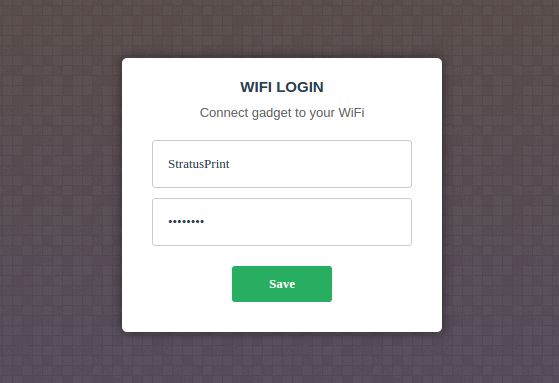
\includegraphics[scale=0.25]{images/wifi-login.png}
    \end{center}
    \end{enumerate}

  \section{Sensors}
  \subsection{Node Pinout}
  \begin{center}
        \includegraphics[scale=0.05]{images/node-pin-out.png}
  \end{center}
    \subsection{Job Button}
      The "Job Button" is a momentary push button that tells the hub that the bed
      is clear and it okay to start the next print. This is to provide an easy way
      for someone to clean the print bed and continue the print queue.\\

      \textbf{Operation}\\
      Once a print is complete this button will blink repeatedly until it is pressed.
      When the button is pressed it tells the hub its clear to start the next job in the
      print queue.\\

      \textbf{Wiring Diagram}\\
            \begin{center}
      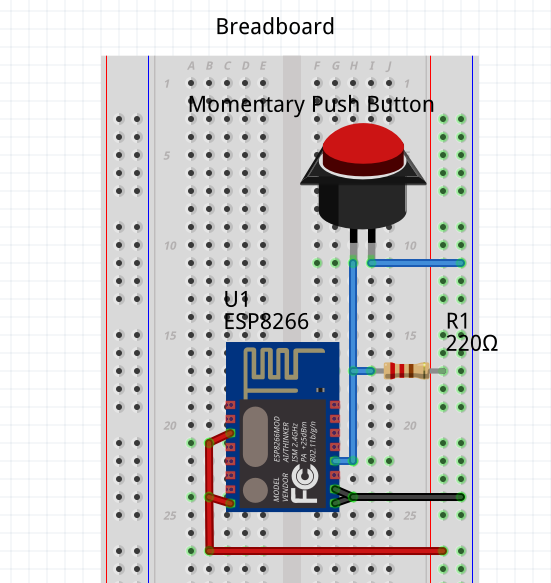
\includegraphics[scale=0.25]{images/job-cir.png}
      \end{center}
    \subsection{Temperature and Humidity}
      The temperature and humidity sensor will report the current room conditions. It
      can detect dangerous conditions for 3D printing and act as an early warning system
      if the conditions may lead to print.\\

      \textbf{Wiring Diagram}\\
            \begin{center}
      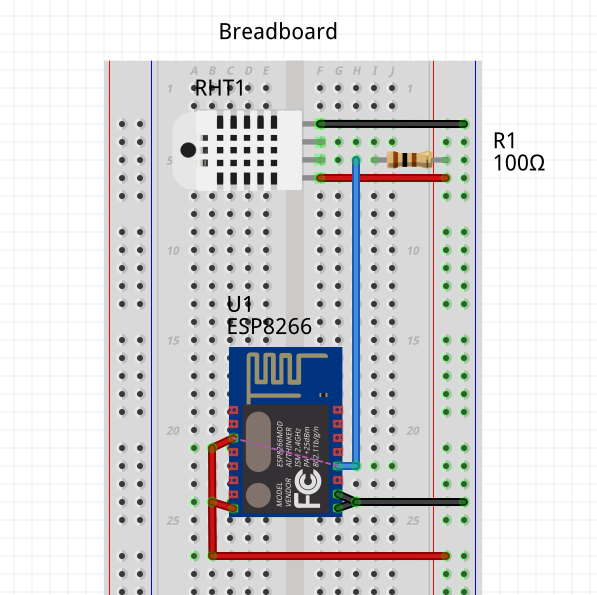
\includegraphics[scale=0.25]{images/temp-diagram.png}
\end{center}

    \subsection{Door Sensor}
      The door sensor is a magnetic switch mounted to the entrance of the printing lab.
      This allows for detection of an open or closed door. Which may affect printing conditions.\\

      \textbf{Wiring Diagram}\\
      \begin{center}
        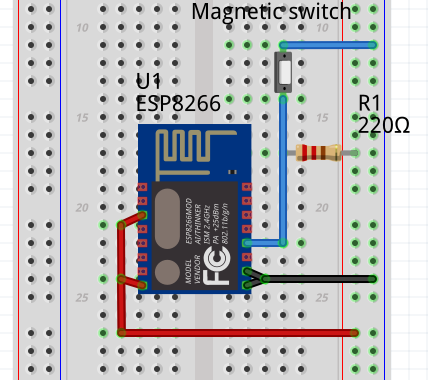
\includegraphics[scale=0.25]{images/door-cir.png}
        \end{center}
    \subsection{Additional Sensors}
      The nodes where set up to be universal and by that are compatible with
      many sensors because of this the nodes come with a breadboard so they can
      easily be reconfigured.\\
\newpage
  \section{Troubleshooting}
  \subsection{Reset}
  Turn the switch the the off position and unplug the node.
  \subsection{Node is not connecting to the hub}
  \begin{enumerate}
    \item Ensure the node has the correct wifi credentials. If the default is not
    working make sure the password hasn't been changed.
    \item If the node seems to be connected and isn't communication hard reset and re-connect.
  \end{enumerate}
  \subsection{Node is connected but no data is being sent from the sensors}
  Make sure the sensors are connected correctly you can reference the wiring diagrams
  in this manual.


\end{document}
